% Plantilla latex para publicación de artículo científico en la revista "SOE"
%
% @autor {Juan Carlos Peinado Pereira}
% @correo {juanpeinado@uagrm.edu.bo}
% @año 2025
% @versión 1.0
% @licencia CC BY 4.0
%
% Se agradecen sus comentarios, contribuciones, reporte de bugs y la difusión de esta plantilla.

% Tipo de documento ytamaño de letra
\documentclass[10pt,twocolumn,a4paper]{article}

% Ajuste de lenguaje
\usepackage[spanish, english]{babel}

% Tamaño de página y margenes
\usepackage[letterpaper, top=2.5cm,bottom=3.5cm, left=3cm, right=2.5cm, marginparwidth=1.75cm]{geometry}

% Permite manejo de ecuaciones y símbolos matemáticos
\usepackage{amsmath, amssymb, amsthm, amsfonts}

% Permite el manejo de caracteres especiales en el español
\usepackage[utf8]{inputenc} 
\usepackage[T1]{fontenc}

% Permite el manejo de citas bibliográficas
\usepackage[backend=biber, style=apa, natbib=true]{biblatex}
\usepackage{csquotes}
% Permite el manejo de citas bibliográficas
\addbibresource{referencias.bib}
% Permite el manejo de citas bibliográficas
%\usepackage{cite}

% Permite manejo de la norma APA Apacite referencias bibliográficas
%\usepackage{apacite}

% Paquete para agregar imágenes
\usepackage{graphicx}

% Fuente principal del texto: Times
\usepackage{mathptmx}

% Permite el manejo de caracteres especiales en el español
\usepackage[utf8]{inputenc} 
\usepackage[T1]{fontenc}

% Subrayado de textos
\usepackage[normalem]{ulem}

% Permite justificar el texto
\usepackage{ragged2e}

% Personalizar los encabezados y pies de página
\usepackage{fancyhdr}
\pagestyle{fancy}
\setlength{\headheight}{36.2396pt}
\addtolength{\topmargin}{-24.2396pt}

% Ruta para imagenes
\graphicspath{{image/}}

% Ajusta la sangría
\setlength{\parindent}{1cm}

% Ajusta el espacio entre renglones
\setlength{\parskip}{0.5cm}

% Paquete para hipervinculos (debe ir después de cite y apacite)
\usepackage{hyperref}
\hypersetup{
    colorlinks=true,
    linkcolor=black,
    urlcolor=black,
    citecolor=black
}
\usepackage{listings} 
\usepackage{xcolor}
\definecolor{codegreen}{rgb}{0,0.6,0}
\definecolor{codegray}{rgb}{0.5,0.5,0.5}
\definecolor{codepurple}{rgb}{0.58,0,0.82}
\definecolor{backcolor}{rgb}{0.95,0.95,0.92}

\lstdefinestyle{mystyle}{
	backgroundcolor=\color{backcolor},
	commentstyle=\color{codegreen},
	keywordstyle=\color{magenta},
	numberstyle=\color{codegray},
	stringstyle=\color{codepurple},
	basicstyle=\ttfamily\footnotesize
}

% Headers config
% Cambiar Volumen, Numero y páginas
\lhead{
    Fronteras Tecnologicas, Febrero 20xx, Vol. x, No. x, páginas xx – xx\\Disponible en línea para descarga en: \href{https://github.com/profjcp/Articulos/}{https://github.com/profjcp/Articulos/}\\ISSN: xx-xx, Postgrado de ingeniería en Ciencias de la Computación y Telecomunicaciones, UAGRM
}
\rhead{
    
\includegraphics[width=1.0cm]{logo}}
\headsep=60pt

% Información del artículo
\title{\Huge Latex una herramienta a disposición del investigador\\}
\author{\Large {1\textsuperscript{st}Juan Carlos Peinado Pereira}}
\date{\normalsize Posgrado SOE - UAGRM\\
\textit{jcpeinado@soe.uagrm.edu.bo}\\
Santa Cruz de la Sierra, Bolivia \\
https://orcid.org/0009-0009-9117-2441}


\begin{document}
\maketitle

\selectlanguage{spanish}
\begin{abstract}
    \textit{\normalsize Este artículo examina el uso de LaTeX como herramienta para la investigación, destacando sus ventajas sobre los procesadores de texto tradicionales. 
    Se enfoca en la precisión tipográfica, el manejo de matemáticas, la gestión de referencias y la estructura de documentos. 
    El autor argumenta que LaTeX mejora la calidad y eficiencia en la producción de documentos científicos, especialmente en ciencias de la computación. El texto presenta una plantilla base en LaTeX para investigadores, junto con una comparativa entre Word y LaTeX.
    Se concluye que LaTeX eleva el prestigio académico y facilita la difusión de la investigación, aunque requiere capacitación inicial.} 
    \vspace{0.5cm}

    \textbf{Palabras clave:} Procesador de texto, Herramientas de investigación, Tipografía, Gestión de referencial, LaTeX.
\end{abstract}


\selectlanguage{english}
\begin{abstract}
    \textit{\normalsize This article examines the use of LaTeX as a research tool, highlighting its advantages over traditional word processors. 
    It focuses on typographical accuracy, mathematics, reference management, and document structure. 
    The author argues that LaTeX improves the quality and efficiency in the production of scientific documents, especially in computer science. 
    The text presents a base LaTeX template for researchers, along with a comparison between Word and LaTeX. 
    It is concluded that LaTeX increases academic prestige and facilitates the dissemination of research, although it requires initial training.}    
    \vspace{0.5cm}

    \textbf{Keywords:} Word processor, Research tools, Typography, Reference management, LaTeX.
\end{abstract}

\selectlanguage{spanish}

    \section{Introducción}

LaTeX, creado por Donald Knuth, es un programa de composición tipográfica que se ha convertido en el estándar de facto para la publicación de artículos científicos y libros académicos en campos como matemáticas y física \parencite{knuth1997art}.
A diferencia de los procesadores de texto tradicionales, LaTeX ofrece precisión y control tipográfico, manejo excepcional de matemáticas y símbolos, gestión eficiente de referencias y citas, estructura y organización de documentos, portabilidad y compatibilidad. 
Ejemplos: Universidades de renombre como el MIT y Stanford, organizaciones científicas como la Sociedad Americana de Física (APS), utilizan LaTeX para sus publicaciones.
\textbf{¿Qué es Latex?}\\
TeX es un programa de composición tipográfica desarrollado por Donald Knuth para su obra maestra The Art of Computer Programming. 
Su función es transformar un archivo de texto plano en un documento de alta calidad, optimizado para impresión y visualización en pantalla.\textcite{poley2000latex} 
Sobre esta base, se creó LaTeX, un sistema de macros diseñado para facilitar el uso de TeX y automatizar tareas comunes de formato.\\ 
LaTeX se ha convertido en un referente para la publicación académica en disciplinas como matemáticas y física, debido a su capacidad para generar documentos de gran precisión tipográfica y a la calidad excepcional de sus fuentes en el ámbito del software libre.\\
Estas son algunas de las principales razones por las que LaTeX es tan valioso en este campo:
\begin{enumerate}  
    \item Precisión y control tipográfico:
    \begin{enumerate}
        \item Calidad de la presentación: LaTeX ofrece un control preciso sobre la tipografía, el espaciado, la alineación y otros detalles de diseño, lo que resulta en documentos con una apariencia profesional y pulcra.
        \item Énfasis en el contenido: Al separar el contenido del formato, LaTeX permite a los investigadores concentrarse en la sustancia de su trabajo, dejando que el sistema se encargue de la presentación. 
    \end{enumerate}
    \item Manejo excepcional de matemáticas y símbolos:
    \begin{enumerate}
        \item Notación matemática avanzada: LaTeX facilita la escritura de ecuaciones complejas, fórmulas y símbolos matemáticos con una claridad y precisión inigualables.
        \item Estándar en la comunidad científica: LaTeX se ha convertido en el estándar para la publicación de artículos científicos y técnicos, especialmente en campos como las matemáticas, la física y la informática.  
    \end{enumerate}
    \item Gestión eficiente de referencias y citas:
    \begin{enumerate}
        \item Automatización de referencias: LaTeX simplifica la gestión de referencias bibliográficas, citas y notas al pie de página, lo que ahorra tiempo y reduce errores.
        \item Consistencia y precisión: LaTeX garantiza la consistencia y precisión en el formato de las referencias, lo cual es crucial para la credibilidad de la investigación.
    \end{enumerate}
	\item Estructura y organización de documentos:
	\begin{enumerate}
        \item Organización jerárquica: LaTeX facilita la organización de documentos extensos en secciones, subsecciones, capítulos y otras estructuras jerárquicas.
        \item Generación automática de índices y tablas de contenido: LaTeX puede generar automáticamente índices, tablas de contenido y listas de figuras y tablas, lo que facilita la navegación y la consulta de documentos.  
    \end{enumerate}
	\item Portabilidad y compatibilidad:
	\begin{enumerate}
        \item Independencia de plataforma: Los documentos LaTeX son independientes de la plataforma, lo que significa que se pueden crear y visualizar en diferentes sistemas operativos sin perder calidad ni formato.
        \item Formatos de salida versátiles: LaTeX permite generar documentos en diversos formatos, como PDF, PostScript y HTML, lo que facilita su distribución y publicación en diferentes medios.   
    \end{enumerate}
    \item Comunidad y recursos:
    \begin{enumerate}
        \item Amplia comunidad de usuarios: LaTeX cuenta con una gran comunidad de usuarios y desarrolladores que ofrecen apoyo, recursos y paquetes adicionales para extender sus funcionalidades.
        \item Documentación exhaustiva: LaTeX dispone de una documentación completa y detallada, así como de numerosos tutoriales y cursos en línea para aprender a utilizarlo.  
    \end{enumerate}
\end{enumerate} 
 
{\raggedleft \textbf{¿Quienes emplean Latex?}}

{\raggedleft \textbf{Instituciones que utilizan LaTeX:}}

\begin{itemize}
	\item Universidades de renombre: Universidades líderes como el MIT, Stanford, Harvard, Oxford y Cambridge, entre muchas otras, utilizan LaTeX para la preparación de tesis, artículos y otros documentos académicos.
	\item Institutos de investigación: Institutos como el CERN, el Instituto Max Planck, el CNRS y el Instituto Nacional de Estándares y Tecnología (NIST) también emplean LaTeX para sus publicaciones.
	\item Organizaciones científicas: Organizaciones como la Sociedad Americana de Física (APS), la Asociación para la Maquinaria de la Computación (ACM) y la Sociedad de Matemáticas Aplicadas e Industriales (SIAM) utilizan LaTeX como estándar para sus publicaciones.
\end{itemize}

{\raggedleft \textbf{Publicaciones que utilizan LaTeX como estándar:}}

\begin{itemize}
	\item Revistas científicas: La mayoría de las revistas científicas de alto impacto en áreas como física, matemáticas, informática, ingeniería y ciencias de la computación requieren que los manuscritos se presenten en formato LaTeX.
	\item Actas de conferencias: Las actas de conferencias de prestigio en ciencias de la computación y otras áreas técnicas a menudo utilizan LaTeX para garantizar la uniformidad y calidad de los documentos.
	\item Libros académicos: Muchos libros de texto y obras de referencia en ciencias y matemáticas se publican utilizando LaTeX debido a su capacidad para manejar notaciones matemáticas complejas y producir documentos de alta calidad.
\end{itemize}

{\raggedleft \textbf{Fuentes de datos que emplean LaTeX:}}
\begin{itemize}
	\item Google Scholar: Google Scholar indexa artículos científicos y otros documentos académicos en una amplia variedad de disciplinas. Muchos de estos documentos están escritos en LaTeX, especialmente en áreas como matemáticas, física e informática.
	\item Scopus: Scopus es una base de datos bibliográfica de Elsevier que indexa una gran cantidad de literatura científica, incluyendo artículos de revistas, actas de conferencias y libros. Muchos de los documentos indexados en Scopus están escritos en LaTeX.
	\item Web of Science: Web of Science es otra base de datos bibliográfica ampliamente utilizada que indexa publicaciones científicas de diversas disciplinas. Al igual que Scopus, muchos de los documentos indexados en Web of Science están escritos en LaTeX.
\end{itemize}

\newpage % Agrega o elimina estos saltos de página de acuerdo a tus necesidades.
\vspace{0.5cm}

    \section{Resultados}
    El estudio destaca las numerosas ventajas de LaTeX para investigadores, incluyendo su capacidad para generar documentos con calidad tipográfica superior, manejo eficiente de fórmulas matemáticas y símbolos complejos, y automatización en la gestión de referencias y citas bibliográficas. 
    Estas características son especialmente valiosas en la investigación en ciencias de la computación, donde la precisión y presentación profesional son fundamentales. 
    Además, se proporcionará una plantilla base como apoyo a los investigadores de la unidad de posgrado SOE.
    \subsection{Fases a tomar en cuenta para la elaboración de una plantilla base en Latex :}
    
{\raggedleft \textbf{Definir los requisitos:}}
    \begin{enumerate}
        \item Tipo de documentos: Determina qué tipo de documentos se crearán con la plantilla (tesis, artículos, presentaciones, informes, etc.). Cada uno tendrá requisitos específicos de formato.
        \item Normativa de la SOE: Investiga si la unidad de posgrado tiene lineamientos de formato específicos (márgenes, tamaño de letra, espaciado, etc.).
        \item Estilo de citación: Define el estilo de citación requerido (APA, MLA, Chicago, etc.) y los paquetes de LaTeX necesarios para implementarlo.
        \item Elementos obligatorios: Identifica los elementos que deben estar presentes en todos los documentos (portada, índice, resumen, bibliografía, etc.).
    \end{enumerate}
    
{\raggedleft \textbf{Estructura básica de la plantilla:}}
    \begin{enumerate}
        \item Clase de documento: Elige la clase de documento adecuada (article, book, report, beamer, etc.).
        \item Paquetes esenciales: Incluye los paquetes básicos para el manejo de idiomas, codificación de caracteres, matemáticas, gráficos y otros elementos comunes.
        \item Definición de comandos: Crea comandos personalizados para abreviar tareas repetitivas (encabezados, pies de página, formatos de texto, etc.).
        \item Diseño de la portada: Diseña la estructura de la portada, incluyendo el logo de la SOE, el título del documento, el autor, la fecha y otros datos relevantes.
    Configuración de márgenes y encabezados: Establece los márgenes, encabezados y pies de página según la normativa de la SOE.
    \end{enumerate}

{\raggedleft \textbf{Elementos específicos de la plantilla:}}
    \begin{enumerate}
        \item Estilo de citación: Configura el estilo de citación utilizando paquetes como biblatex o natbib.
        \item Tipografía: Define la tipografía para el cuerpo del texto, los títulos, las secciones y otros elementos.
        \item Numeración de páginas: Configura la numeración de páginas (arábigos, romanos, etc.) y su ubicación.
        \item Tablas y figuras: Crea estilos para la presentación de tablas y figuras, incluyendo leyendas y referencias cruzadas.
        \item Código fuente: Incluye un estilo para la presentación de código fuente, resaltando la sintaxis y utilizando fuentes monoespaciadas.
        \item Matemáticas: Asegúrate de que la plantilla maneje correctamente las ecuaciones y símbolos matemáticos.
    \end{enumerate}
    
{\raggedleft \textbf{Personalización y refinamiento:}}
    \begin{enumerate}
    
        \item Colores y logotipos: Incorpora los colores y logotipos de la SOE.
        \item Fuentes personalizadas: Utiliza fuentes específicas si la unidad de posgrado lo requiere.
        \item Diseño de secciones: Define el diseño de las secciones, subsecciones y otros elementos jerárquicos.
        \item Ejemplos de uso: Incluye ejemplos de cómo utilizar la plantilla para diferentes tipos de documentos.
    \end{enumerate}
    
{\raggedleft \textbf{Documentación y distribución:}}
    \begin{enumerate}
        \item Manual de usuario: Crea un manual de usuario que explique cómo utilizar la plantilla y personalizarla.
        \item Plantilla en línea: Considera la posibilidad de crear una plantilla en línea en Overleaf para facilitar su uso y colaboración.
        \item Repositorio de la plantilla: Publica la plantilla en un repositorio (GitHub, GitLab, etc.) para que esté disponible para todos los miembros de la SOE. \url{https://github.com/profjcp/Articulos/}
    \end{enumerate}
    \subsection{Esquema de compilacion de LaTex:}
    El proceso de compilación de un documento LaTeX es esencial para transformar el código fuente en un documento final formateado. 
    A diferencia de los procesadores de texto tradicionales, LaTeX no formatea el documento directamente mientras se escribe. 
    En cambio, se utilizan comandos y etiquetas para marcar la estructura y el contenido del documento, y luego un programa llamado "motor de LaTeX" se encarga de procesar estas instrucciones y generar el documento final.
    
    \textbf{Aquí hay algunos puntos clave sobre el proceso de compilación:}

    Código fuente: El documento LaTeX comienza como un archivo de texto con extensión .tex. Este archivo contiene el texto del documento, así como los comandos y etiquetas que controlan el formato, la estructura y otros elementos.

    Motor de LaTeX: El motor de LaTeX es el programa que interpreta el código fuente y genera el documento formateado. Hay varios motores de LaTeX disponibles, como pdfTeX, XeTeX y LuaTeX, cada uno con sus propias características y capacidades.

    Proceso de compilación: El proceso de compilación generalmente implica varios pasos. Primero, el motor de LaTeX lee el archivo .tex y procesa las instrucciones. Luego, genera uno o varios archivos intermedios, como archivos .dvi (Device Independent) o .pdf (Portable Document Format). Finalmente, estos archivos intermedios se utilizan para crear el documento final en el formato deseado.

    Archivos auxiliares: Durante el proceso de compilación, LaTeX también puede generar archivos auxiliares que contienen información sobre el documento, como la tabla de contenidos, la bibliografía y las referencias cruzadas. Estos archivos se utilizan en compilaciones posteriores para garantizar la coherencia del documento.

    Iteraciones: En algunos casos, puede ser necesario compilar el documento varias veces para que todos los elementos se formateen correctamente. Por ejemplo, si el documento contiene referencias cruzadas, es posible que sea necesario compilarlo dos veces para que los números de página y las referencias se actualicen correctamente.

    Una vez que se ha completado el proceso de compilación, se puede ver el documento final en un visor de PDF o imprimirlo. El documento resultante tendrá una calidad tipográfica profesional y se verá igual independientemente del sistema operativo o el software utilizado para visualizarlo.


    El siguiente esquema muestra el proceso de compilación de un documento LaTeX:
    \begin{figure}[!ht]
        \centering
        \makebox[\linewidth][c]{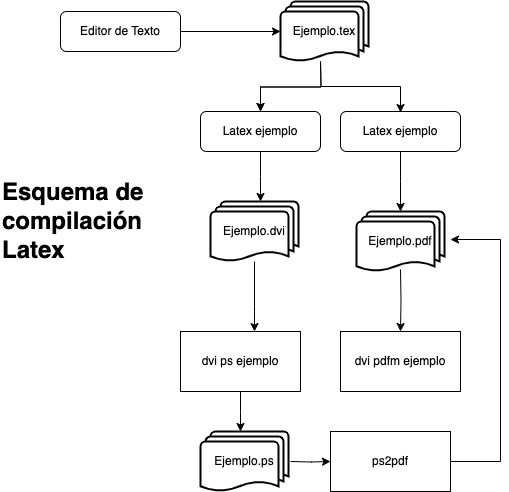
\includegraphics[width=0.5\linewidth]{LatexD.png}}%
        \caption{Esquema de compilacion de LaTex}
        \label{fig:LatexD}
    \textit{nota: En la figura se muestra el proceso de compilación de un documento LaTeX. El archivo fuente (.tex) se compila utilizando un motor LaTeX (pdfLaTeX, XeLaTeX, LuaLaTeX) para generar un archivo PDF. El proceso puede requerir varias pasadas para resolver referencias cruzadas, citas bibliográficas y otros elementos.}
    \end{figure} 
    
    \subsection{Propuesta de plantilla base en Latex}
    Al adoptar LaTeX y utilizar la plantilla base propuesta, los investigadores de la unidad de posgrado SOE podrán producir documentos de alta calidad que cumplan con los estándares internacionales de publicación. 
    Esto no solo facilitará la difusión de sus investigaciones, sino que también contribuirá a elevar el prestigio académico de la unidad de posgrado.\\
    Nota: La platilla que se muestra a continuación no cuenta con el formato UTF8 que ayuda a la visualización de caracteres especiales en español, sin embargo, se puede agregar en el preámbulo del documento.\\
    Plantilla ejemplo para la creación de artículos científicos en LaTeX:
    \begin{lstlisting}[style=mystyle]
      
        %%%%%%%%%%%%%%%%%%%%%%%%%%%%%%%%%%%%%%%%%%%%%%%%
        % @autor {Juan Carlos Peinado Pereira}
        % @correo {juanpeinado@uagrm.edu.bo}
        % @ano 2025
        % @version 1.0
        % @licencia CC BY 4.0
        %%%%%%%%%%%%%%%%%%%%%%%%%%%%%%%%%%%%%%%%%%%%%%%%
    
        % Se agradecen sus comentarios, contribuciones, y la difusion de esta plantilla
        
        % Tipo de documento y tamano de letra
        \documentclass[10pt]{article}
        
        % Ajuste de lenguaje
        \usepackage[spanish, english]{babel}
        
        % Tamano de pagina y margenes
        \usepackage[letterpaper, top=2.5cm,bottom=3.5cm, left=3cm, 
        right=2.5cm, marginparwidth=1.75cm]{geometry}
        
        % Permite manejo de ecuaciones y simbolos matematicos
        \usepackage{amsmath, amssymb, amsthm, amsfonts}
        
        % Permite el manejo de citas bibliograficas
        \usepackage{cite}
        
        % Permite manejo de la norma APA Apacite referencias bibliograficas
        \usepackage{apacite}
        
        % Paquete para agregar imagenes
        \usepackage{graphicx}
        
        % Fuente principal del texto: Times
        \usepackage{mathptmx}
        
        % Permite el manejo de caracteres especiales en el espanol
        \usepackage[utf8]{inputenc} 
        \usepackage[T1]{fontenc}
        
        % Subrayado de textos
        \usepackage[normalem]{ulem}
        
        % Personalizar los encabezados y pies de pagina
        \usepackage{fancyhdr}
        \pagestyle{fancy}
        
        % Ruta para imagenes
        \graphicspath{{image/}}
        
        % Ajusta la sangria
        \setlength{\parindent}{1cm}
        
        % Ajusta el espacio entre renglones
        \setlength{\parskip}{0.5cm}
        
        % Paquete para hipervinculos (debe ir despues de cite y apacite)
        \usepackage{hyperref}
        \hypersetup{
            colorlinks=true,
            linkcolor=black,
            urlcolor=black,
            citecolor=black
        }
        
        % Headers config
        % Cambiar Volumen, Numero y paginas
        \lhead{
            Fronteras Tecnologicas, Febrero 20, Vol.x, No.x, paginas \\ href:xx\\ISSN:x}
        \rhead{
            
\includegraphics[width=1.2cm]{logo}}
        \headsep=60pt
        
        % Informacion del articulo
        \title{\Huge Titulo de investigacion\\}
        \author{\Large Autores de la publicacion}
        \date{\normalsize Datos de la Institucion de adscripcion de los autores.\\
        \textit{xxxx@soe.uagrm.edu.bo}\\
        Santa Cruz de la Sierra, Bolivia \\
        https://orcid.org/0009-0009-9117-2441}
        
        
        \begin{document}
        \maketitle
        \end{doocument}
        
    \end{lstlisting}

    %\begin{figure}[ht]
    %\centering
    %\makebox[\linewidth][c]{\includegraphics[width=1\linewidth]{Figures/PlantillaLatex.png}}%
    %\caption{Plantilla para Artículos Científicos}
    %label{fig-2}
    %\end{figure}
    
    Invitamos a los investigadores de la unidad de posgrado SOE a adoptar LaTeX y a utilizar la plantilla base proporcionada. 
    Para aquellos que deseen aprender a utilizar LaTeX, se ofrecerán un repositorio en GitHub con toda la documentación necesaria para iniciar en LaTeX. 
    Estamos seguros de que esta iniciativa contribuirá a mejorar la calidad y la eficiencia de la investigación en nuestra unidad de posgrado.  
    
Una vez que se ha aplicado la plantilla base propuesta en Latex en la ecritura de este documento, se obtienen los siguientes resultados:
    \begin{enumerate}
        \item Control preciso sobre la tipografía y el espaciado, tambien en la selección de funtes y alineados.
        \item Estructura clara y consistente en todo el documento, con una variedad de plantillas y estilos predefinidos.
        \item Gestión eficiente de citas con paquetes como biblatex y natbib, con una amplia variedad de estilos de citación.
        \item Integración fluida de gráficos generados con herramientas externas, como TikZ o pgfplots.
        \item Facilidad para la creación de tablas complejas con un código legible.
        \item Facilidad para la escritura de ecuaciones complejas con un código legible.
        \item Facilidad para la automatización de la generación de bibliografías y la inserción de citas.
    \end{enumerate}
    Todas estas características convierten a LaTeX en una herramienta pertinente para los investigadores de la Unidad de Posgrado SOE, ya que permite la creación de documentos científicos con un alto nivel de precisión, claridad y profesionalismo. 
    Su capacidad para gestionar referencias bibliográficas, integrar ecuaciones matemáticas, tablas y gráficos con formato consistente, así como su compatibilidad con repositorios colaborativos como GitHub, facilita el trabajo académico y promueve buenas prácticas en la escritura científica.\\
    A continuación se muestra un cuadro comparativo de la plantilla realizada entre word vs LaTeX, después de haber aplicado el formato base en Latex segun las normativa expuestas por SOE.  \ref{tab:Comparativas}.

\vspace{0.5cm}
    \begin{table}[h!]
        \centering
        \resizebox{16cm}{!}{
            \begin{tabular}{|c|c|c|}
            \hline
            \textbf{Aspectos} & \textbf{Word} & \textbf{Latex} \\ \hline
            \textbf{Tipografía}      &         &                   \\ \hline
            {Calidad}         & Generalmente buena, pero limitada en opciones de personalización.          & Excelente, con control preciso sobre la tipografía y el espaciado.\\ \hline
            {Control}         & Limitado a las opciones predefinidas.          & Amplio control sobre todos los aspectos tipográficos.                  \\ \hline
            {Consistencia}    & Puede ser difícil mantener la consistencia en documentos largos.          & Garantiza la consistencia en todo el documento.                  \\ \hline
            \textbf{Formatos}        &         &                   \\ \hline
            {Predefinidos}    & Ofrece una variedad de plantillas y estilos predefinidos.          & Permite el uso de clases de documentos y paquetes para diferentes formatos.\\ \hline
            {Personalización} & Permite la personalización, pero puede ser complejo y llevar mucho tiempo.          & Ofrece una gran flexibilidad para la personalización.                \\ \hline
            {Estructura}      & Se basa en una interfaz WYSIWYG (lo que ves es lo que obtienes).          & Se basa en comandos y etiquetas para estructurar el documento.                  \\ \hline
            \textbf{Fuentes}         &         &                   \\ \hline
            {Variedad}        & Ofrece una variedad de plantillas y estilos predefinidos.          & Amplia variedad de fuentes disponibles, especialmente para matemáticas y símbolos.\\ \hline
            {Control}         & Control limitado sobre la selección y el uso de fuentes.          & Control preciso sobre la selección y el uso de fuentes.                \\ \hline
            \textbf{Citas bibliográficas}         &         &                   \\ \hline
            {Gestion}         & Ofrece herramientas para la gestión de citas, pero pueden ser limitadas.          & Ofrece una gestión eficiente de citas con paquetes como biblatex y natbib.                 \\ \hline
            {Estilo}          & Permite el uso de diferentes estilos de citación.          & Permite el uso de una amplia variedad de estilos de citación.\\ \hline
            {Automatización}  & Ofrece cierta automatización, pero puede requerir intervención manual.          & Automatiza la generación de bibliografías y la inserción de citas.                \\ \hline
            \textbf{Gráficos}        &         &                   \\ \hline
            {Creación}        & Permite la creación de gráficos básicos dentro del documento.          & Requiere el uso de herramientas externas (como TikZ o pgfplots) para generar gráficos de alta calidad.                \\ \hline
            {Personalización} & Ofrece opciones de personalización limitadas.          & Ofrece un alto grado de personalización para la apariencia de los gráficos.\\ \hline
            {Integración}     & Integración sencilla de gráficos creados en otras aplicaciones.          & Integración fluida de gráficos generados con herramientas externas.              \\ \hline
            \textbf{Tablas}          &         &                   \\ \hline
            {Creación}        & Permite la creación de tablas con una interfaz gráfica.        & Se crean mediante comandos y entornos.                \\ \hline
            {Formato}         & Ofrece opciones de formato básicas.          & Permite un control preciso sobre el formato y la apariencia de las tablas.\\ \hline
            {Complejidad}     & Puede ser complicado crear tablas complejas con múltiples filas y columnas.          & Facilita la creación de tablas complejas con un código legible.              \\ \hline
            \textbf{Expresiones matemáticas}          &         &                   \\ \hline
            {Escritura}        & Permite la inserción de ecuaciones con un editor de ecuaciones.        & Se escriben utilizando comandos y símbolos.                \\ \hline
            {Calidad}         & La calidad de las expresiones matemáticas puede ser limitada.         & Produce expresiones matemáticas de alta calidad con una tipografía profesional.\\ \hline
            {Complejidad}     & Puede ser complicado escribir ecuaciones complejas.          & Facilita la escritura de ecuaciones complejas con un código legible.              \\ \hline
            \end{tabular}
        }
        \caption{Comparativa entre Word y Latex, en la aplicacion de plantillas base.}
        \label{tab:Comparativas}
    \end{table}
\vspace{0.5cm}
    
    \section{Conclusiones}
    La adopción de LaTeX en la escritura de este documetno ha permitido mejorar significativamente la calidad tipográfica en la investigación presentada. 
    Lo que se traduce en una presentación más profesional y legible de los resultados. Sin embargo, la curva de aprendizaje inicial puede representar un desafío para algunos investigadores, lo que requiere la implementación de programas de capacitación y soporte técnico.
    Por este motivo es que se propone la creación de un repositorio en GitHub con toda la documentación necesaria para iniciar en LaTeX, así como la organización de talleres y seminarios para capacitar a los investigadores en el uso de esta herramienta.
    Para un futuro trabajo se propone la creación de una plantilla en línea en Overleaf para facilitar su uso y colaboración, así como la publicación de la plantilla en un repositorio (GitHub, GitLab, etc.) para que esté disponible para todos los miembros de la unidad de posgrado SOE.

    Se concluye que LaTeX facilita la estructuración lógica y la organización eficiente de documentos extensos, un aspecto particularmente valioso en la investigación académica. 
    La capacidad de LaTeX para separar el contenido del formato permite a los investigadores concentrarse en el desarrollo de sus ideas, delegando en el sistema la tarea de dar forma al documento. 
    La generación automática de índices y tablas de contenido simplifica la navegación del lector a través del texto, mejorando la accesibilidad a la información.

%\nocite{*}
%\bibliographystyle{apacite}
\printbibliography
%\bibliography{referencias}

\end{document}